\chapter{Gestión del proyecto}


En este capítulo se explican el modelo de proceso seleccionado y las distintas etapas por las que ha pasado el este Trabajo Fin de Grado centradose únicamente en los aspectos más importantes. Para profundizar más sobre estos aspectos debe acudir a los anexos.

\section{Modelo de proceso seleccionado}


Este Trabajo Fin de Grado ha surgido una importante evolución desde el primer planteamiento hasta la obtención del sistema final. La primera idea para la evaluación de los algoritmos de recomendaciones era la utilización de un videojuego ya que este podría recolectar datos de forma transparente mientras los usuarios se divertian. El videojuego consistiría en el cumplimiento de misiones en una cuidad basandose en algún videojuego de aventuras como el videojuego Paperboy del año 1985 donde un chico reparte periódicos en una cuidad.

Por esto se ha planteado usar el motor gráfico Unity 5 para el desarrollo del videojuego ya que no tenía sentido desarrollar un videojuego usando simplemente un lenguaje de programación. Pero existía la incertidumbre si todos los requisitos podrían ser implementados. Esto era debido porque por una parte no se conocían de antemano todos los requisitos y por otra no se conocía si el motor gráfico tenía algún tipo de limite. 

Para solucionar estos problemas se ha tomado la decisión de elegir el modelo en espiral como modelo de trabajo. Las actividades de este modelo forman una espiral de tal forma que cada iteración representa un conjunto de actividades. Esto nos permitiría segmentar el trabajo en tareas más pequeñas e ir definiendo los requisitos mientras se desarrollaba el videojuego. De esta manera podríamos evaluar si los requisitos propuestos podrían o no ser implementados con Unity 5. En caso de que el motor gráfico tuviese algún límite tendríamos la capacidad de reorientar el proyecto.

\subsection{Etapa 1}

En la tabla \ref{tabla:requisitosEtapa1} podemos encontrar las tareas que han sido definidas para esta etapa:

\begin{table}[H]
\begin{center}
\begin{tabular}{|p{1.5cm}| p{10.5cm}|}
\hline 
Código & Descripción \\
\hline \hline
RQ-0  & Formación básica con Unity 5\\ \hline
RQ-1  & Establecer puntos en el mapa para que el jugador pueda ir a buscarlos. \\ \hline
RQ-2  & Los puntos establecidos en el requisitos RQ-1 deben de ser extraibles desde un servidor externo\\ \hline
RQ-3  & Establecer una conexión HTTP/JSON entre Unity 5 y un servidor externo. \\ \hline
RQ-4  & Sacar el modelado geométrico de un servidor externo \\ \hline
RQ-5  & El videojugo debe de tener un menú principal \\ \hline
RQ-6  & Investigar si se puede usar Longitud y Latitud con Unity 5 \\ \hline
RQ-7  & Investigar si los edificio generados con CityEngine 2014 son reales o no \\ \hline
RQ-8  & Permitir que el juego se realice sobre mapas de ciudades reales \\ \hline
RQ-9  & Investigar si es posible el desarrollo de videojuego en 3D \\ \hline
\end{tabular}
\caption{Tareas etapa 1}
\label{tabla:requisitosEtapa1}
\end{center}
\end{table}

Como conclusión de esta etapa obtenemos el siguiente resultado:
\begin{itemize}
	\item puede establecerse una conexión con un servidor externo mediante HTTP/JSON (RQ-3). 
	\item pueden establecerse puntos en el mapa para que el jugador pueda ir a buscarlos(RQ-1). 
	\item pueden extraerse puntos desde un servidor externo para que el usuarios pueda ir a buscarlos (RQ-1 y RQ-3).
	\item la realizacion del menú principal del videojuego ha sido posible.
	\item Unity 5 utiliza eje de abscisas. Por lo tanto si queremos usar coordenadas geográficas tenemos que calcular la Longitud y Latitud a partir del eje de coordenadas (x, y, z).
	\item los datos sobre los edificios de OpenStreetMap no están completos.
	\item se ha decido de dejar atrás el modelado 3D ya que se han detectado los siguientes problemas: coste en cuanto a tiempo demasiado grande para el diseño de una ciudad, CityEngine 2014 no interpreta correctamente los datos exportados además no existe ninguna otra herramienta que nos permita la correcta interpretación de los datos (por lo menos yo no podido encontrarla).
\end{itemize}

\subsection{Etapa 2}

En la tabla \ref{tabla:requisitosEtapa2} podemos encontrar las tareas que han sido definidas para esta etapa:

\begin{table}[H]
\begin{center}
\begin{tabular}{|p{1.5cm}| p{10.5cm}|}
\hline 
Código & Descripción \\
\hline \hline
RQ-10 & Investigar como se desarrollan grafos en Unity para la posterior implementación de la IA sobre estos para el movimiento de los vehículos etc. \\ \hline
RQ-11 & Diseñar y desarrollar un mapa del juego\\ \hline
\end{tabular}
\caption{Tareas etapa 2}
\label{tabla:requisitosEtapa2}
\end{center}
\end{table}

Como conclusión de esta etapa obtenemos el siguiente resultado:
\begin{itemize}
	\item Unity 5 dispone de su propio modulo de IA y por lo tanto no hace falta implementar algoritmos de IA para el comportamiento de los objetos dinámicos.
	\item en esta etapa se ha definido el requisito que el juego tiene que funcionar sobre cualquier mapa del mundo. Por lo tanto en la siguiente etapa hay que investigar si es posible la integración de Unity 5 con OpenStreetMap.
\end{itemize}

\newpage

\subsection{Etapa 3}

En la tabla \ref{tabla:requisitosEtapa3} podemos encontrar las tareas que han sido definidas para esta etapa:

\begin{table}[H]
\begin{center}
\begin{tabular}{|p{1.5cm}| p{10.5cm}|}
\hline 
Código & Descripción \\
\hline \hline
RQ-11 & Investigar en que consiste el formato OSM\\ \hline
RQ-12 & Investigar si es posible la integración de OpenStreetMap con Unity\\ \hline
\end{tabular}
\caption{Tareas etapa 3}
\label{tabla:requisitosEtapa3}
\end{center}
\end{table}

Como conclusión de esta etapa obtenemos el siguiente resultado:
\begin{itemize}
	\item Unity 5 no puede ser integrado con OpenStreetMap y no es capaz de renderizar mapas a partir sus datos (ficheros OSM). 
	\item en esta etapa se ha decido reorientar el proyecto por las siguientes razones: Unity 5 no puede ser integrado con OpenStreetMap por lo tanto la única opción para desarrollar un videojuego sobre mapas reales es desarrollando el videojuego desde cero con algún lenguaje como Java y el inconveniente que esto representa es que es demasiado costoso en cuanto a tiempo y dificultad.  
\end{itemize}

\subsection{Etapa 4}

En la tabla \ref{tabla:requisitosEtapa4} podemos encontrar las tareas que han sido definidas para esta etapa:

\begin{table}[H]
\begin{center}
\begin{tabular}{|p{1.5cm}| p{10.5cm}|}
\hline 
Código & Descripción \\
\hline \hline
RQ-12 & instalar mongoDB\\ \hline
RQ-13 & instalar Node.js y NPM\\ \hline
RQ-14 & instalar git\\ \hline
RQ-14 & instalar Java y Apache maven\\ \hline
RQ-16 & Desarrollar y configurar la base de la aplicación con Node.js\\ \hline
RQ-17 & Instalar y configurar Angular.js\\ \hline
RQ-18 & Instalar y configurar OpenLayers.js\\ \hline
RQ-19 & Instalar y configurar Bootstrap\\ \hline
\end{tabular}
\caption{Tareas etapa 4}
\label{tabla:requisitosEtapa4}
\end{center}
\end{table}

\newpage

Como conclusión de esta etapa obtenemos el siguiente resultado:
\begin{itemize}
	\item se han instalado y configurado todas las herramientas y frameworks necesarios para el desarrollo de la aplicación.
\end{itemize}

\subsection{Etapa 5}

En la tabla \ref{tabla:requisitosEtapa5} podemos encontrar las tareas que han sido definidas para esta etapa:

\begin{table}[H]
\begin{center}
\begin{tabular}{|p{1.5cm}| p{10.5cm}|}
\hline 
Código & Descripción \\
\hline \hline
RQ-20 & Definir lo requisitos funcionales y no funcionales de la aplicación\\ \hline
RQ-21 & Desarrollar el front-end\\ \hline
RQ-22 & Deseñar la base de datos\\ \hline
RQ-23 & Diseñar y desarrollar el back-end\\ \hline
RQ-24 & Diseñar y desarrollar el recomendador\\ \hline
RQ-25 & Realizar pruebas funcionales de la aplicación\\ \hline
\end{tabular}
\caption{Tareas etapa 5}
\label{tabla:requisitosEtapa5}
\end{center}
\end{table}

Como conclusión de esta etapa obtenemos el siguiente resultado:
\begin{itemize}
	\item la parte mas costosa de esta etapa ha sido la definición de los requisitos de la aplicación.
	\item una vez definidos los requisitos el resto del trabajo ha sido puramente técnico. 
\end{itemize}


\subsection{Etapa 6}

La última etapa consiste en documentar el trabajo realizado en este Trabajo Fin de Grado.

\newpage

\section{Tiempo dedicado}

Como ya se ha comentado anteriormente, el desarrollo del proyecto se ha realizado siguiendo el modelo en espiral. En esta sección se mostrará el tiempo dedicado y también un cronograma de las diferentes etapas.

\begin{table}[H]
\begin{center}
\begin{tabular}{|c|c|}
\hline 
\noindent{\textbf{Fase}} & \noindent{\textbf{Horas}} \\
\hline \hline
Fase 1 & 54\\ \hline
Fase 2 & 6.5\\ \hline
Fase 3 & 38\\ \hline
Fase 4 & 3.5\\ \hline
Fase 5 & 247\\ \hline
Fase 6 & 42.5\\ \hline
Reuniones & 7\\ \hline
Pruebas de carga & 11.5 \\ \hline
\hline \hline
\noindent{\textbf{Total}} & \noindent{\textbf{410}} \\ \hline
\end{tabular}
\caption{Separación por horas de las distintas fases}
\label{tabla:requisitosEtapa5}
\end{center}
\end{table}
 

\begin{figure}[H]
\centering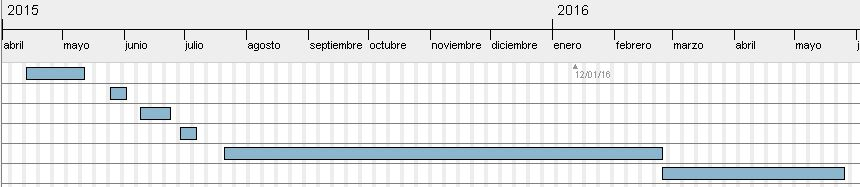
\includegraphics[scale=0.8]{imagenes/gantt.jpg}
\caption{Diagrama de Gantt de las distintas fases del proyecto}
\label{gantt}
\end{figure}
